\chapter{Special Theory of Relativity}
The $20^{\text{th }}$ century saw essentially two major triumphs in physics: the discovery of quantum mechanics and the discovery of relativity.
\section{Reference Frame}
\begin{wrapfigure}{r}{0.40\textwidth}
	\begin{center}
		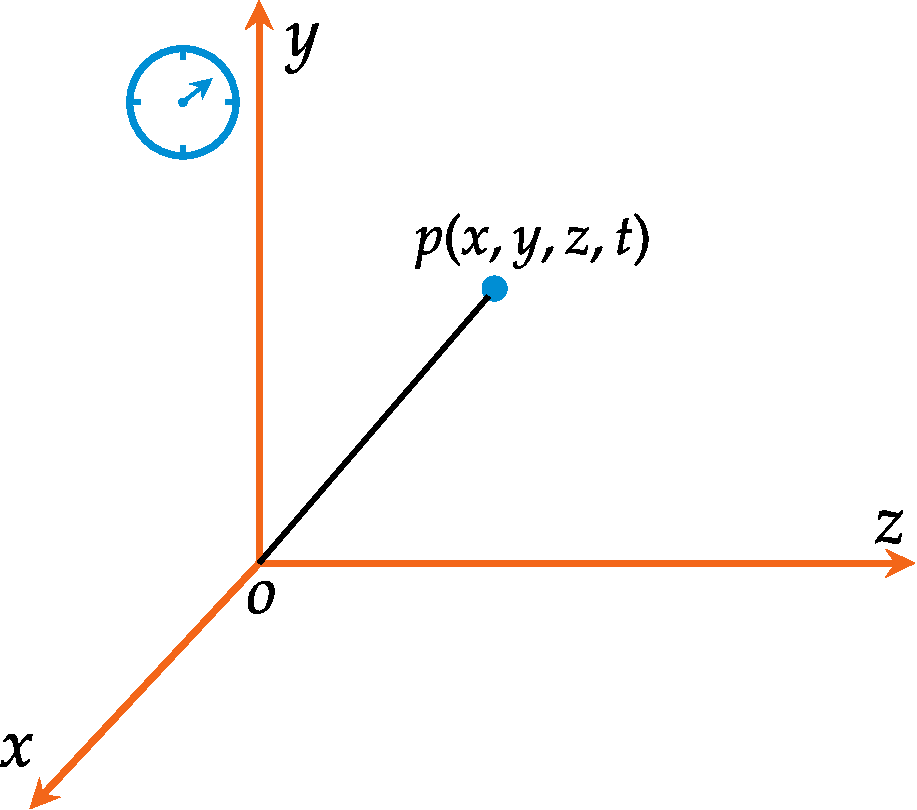
\includegraphics[width=0.25\textwidth]{str1}
	\end{center}
	\caption{Reference Frame}
\end{wrapfigure}
Reference frames are physico-mathematical structures that have the purpose of allowing the objective description, also from a quantitative viewpoint, of physical phenomena that are observed in nature.\\
In order to describe the motion of a particle in space, we need to know its position at different instants of time. This needs the choice of reference body or coordinate system. If we imagine a coordinate system attached to a rigid body and we describe the position of any particle relative to it, then such a coordinate system is called frame of reference. For the location of the objects, the position vectors are drawn from the origin $O$ of the coordinate system . \textbf{A reference frame with four coordinates $\mathrm{x}, \mathrm{y}, \mathrm{z}, \mathrm{t}$ is referred as space-time frame}. The simplest frame of reference is a cartesian coordinate system. 
\subsection{Inertial Frame of Reference}
Inertial frames are frames in which Newton's laws of motion holds true.
It is the one in which the law of inertia holds true i.e., if a particle, subject to no external force, is found to move in a straight line with constant velocity (or to remain at rest), then the coordinate system used for this purpose is called inertial frame.
\begin{align*}
\intertext{We know that according to  Newton's second law of motion,}
F&=\frac{dP}{dt}\\
&=\frac{d(mV)}{dt}
\intertext{If\ $F=0$}
\frac{dV}{dt}&=0
\intertext{Then velocity is constant in inertial frame of reference.}
\end{align*}
Inertial frames are  related by a constant velocity along any axis.  An object is at rest in an inertial frame when it's position in space does not change with time.\\
 
\subsection{Non-Inertial Frame of Reference}
 Accelerated frame of reference in which Newton's law does not hold good.\\\\
 If there is an observer  in a rotating frame then, according to the obeserver a person standing out of his  frame is seems to be accelerating , and then,  according to the observer ,  a force seems to be acting on the person. Then , first law of motion will not be holding in an accelerated frame.
\section{Galilean Transformation } 
An event or physical phenomena, observed simultaneously in two separate reference frames, will have to separate set of coordinates. \textbf{Equation relating two coordinate system  is called transformation equation.} \\
Let $ S $ and $ S^{\prime} $ be two inertial frame of reference with observer at origin $\mathrm{O}$ and $\mathrm{O}^{\prime}$ moving with a relative velocity $y$ along positive direction of $x$.
The Galilean transformation successfully explained the invariance of laws of Newtonian mechanics in different inertial frame. Let the coordinates $(x, t)$ denote the location of an event in the non moving frame $s$ and $\left(x^{\prime}, t^{\prime}\right)$ denote the location of the same event in the moving frame $s^{\prime}$. The Galilean transformation which relates the two coordinate systems is:
\begin{align*}
	x^{\prime} &=x-v t \\
	y^{\prime} &=y \\
	z^{\prime} &=z \\
	t^{\prime} &=t
\end{align*}
\subsubsection{Inverse transformation}
\begin{align*}
	x&=x^{\prime}+v t^{\prime}\\  y&=y^{\prime} \\z&=z^{\prime} \\
	t&=t^{\prime}
\end{align*}
\subsubsection{Velocity transformation}
\begin{align*}
	u_{x}^{\prime}&=u_{x}-v \\u_{y}^{\prime}&=u_{y}\\ u_{z}^{\prime}&=u_{z}
	\intertext { \textbf{Inverse Velocity Transformation }}
	u_{x}&=u_{x}^{\prime}+v \\ u_{y}&=u_{y}^{\prime} \\ u_{z}&=u_{z}^{\prime}
\end{align*}
\subsubsection{Transformation of acceleration}
Let $ a $ and  ${a}^{\prime}$  be the acceleration in ${S}$ and ${S}^{\prime}$ frame of reference.\\
We have, 
\begin{align*}
a^{\prime}&=\frac{d u^{\prime}}{d t}\\&=\frac{d(u-v)}{d t}\hspace{3cm} [\because v=0]\\&=\frac{d u}{d t}-0\\&=a\\
\intertext{$\therefore$ Acceleration is invariant under Galilean transformation.}
\end{align*}
\section{Postulates of Special Theory of Relativity}
Einstein in 1905 , formulated this special theory of relativity on the basis of following postulates:
\begin{enumerate}
	\item \textbf{The laws of physics are same in all inertial frames. This is the principle of relativity.}
	\item \textbf{The speed of light in vacuum is constant and same as observed from all inertial frames. This is known as the principle of constant of speed of light.}
\end{enumerate}

The first postulate implies that not only the laws of mechanics but also that of electrodynamics and optics should be same for all inertial reference systems. There is no privileged frame like ether or absolute space.\\\\
 If Einstein's postulate that the velocity of light is the same in all inertial frames  is correct, then the Galilean transformation is not the correct way to transform space-time coordinates between two inertial frames.einstein showed that, Maxwell's theory is consistent with special relativity whereas, Newtonian mechanics is not, and his modification of these branches of physics into accord.
 \section{Lorentz transformation}
\begin{figure}[H]
	\centering
	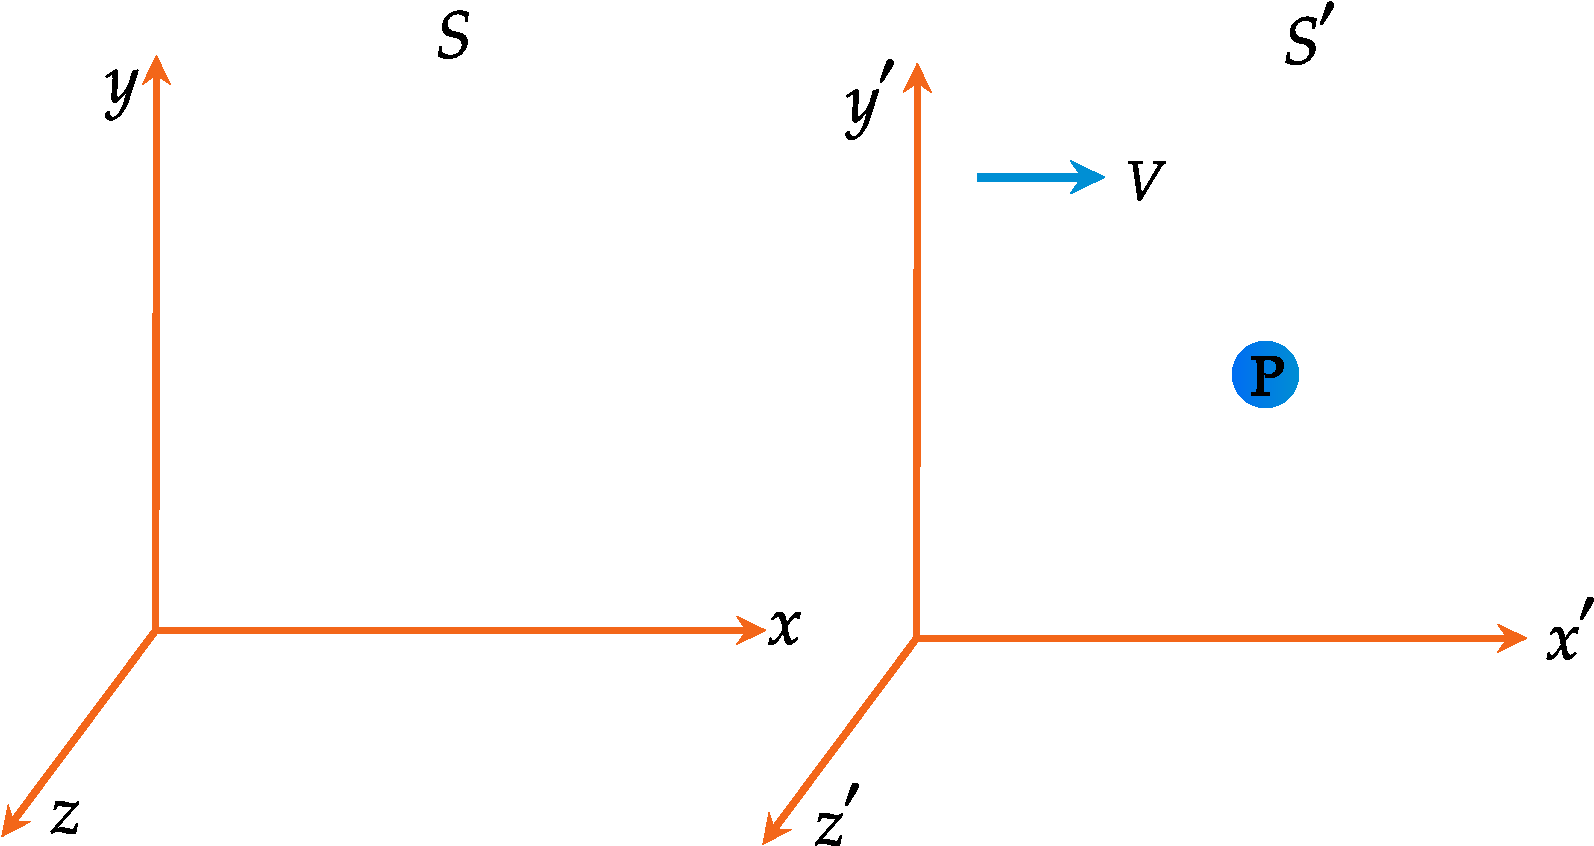
\includegraphics[height=5cm,width=10cm]{lorentz}
	\caption{Lorentz transformation}
	\label{}
\end{figure}
Since the Galilean transformations are inconstitent with some branches of physics we need to replace it with new one. Here we shall derive new equations  using the postulates of special relativity theory and in addition, the assumptio that space and time are homogeneous (All points in space and time are equivalent) \\\\
Our problem can be exactly formulated in the following manner. What are the
values $\mathrm{x}^{\prime}, \mathrm{y}^{\prime}, \mathrm{z}^{\prime}, \mathrm{t}^{\prime}$, of an event with respect to $\mathrm{S}^{\prime}$, when the magnitudes $\mathrm{x}, \mathrm{y}, \mathrm{z}, \mathrm{t}$, of the
same event with respect to $\mathrm{S}$ are given . The relations must be so chosen that the law of the
transmission of light in vacuum is satisfied for one and the same ray of light
 with respect to $\mathrm{S}$ and $\mathrm{S}^{\prime}$. For the relative orientation in space of the co-
ordinate systems , this problem is solved by means of the equations:
\begin{align*}
	x^{\prime} &=\frac{x-v t}{\sqrt{1-\frac{v^{2}}{c^{2}}}} \hspace{2cm} \text{Since,}\ \gamma=\frac{1}{\sqrt{1-v^{2} / c^{2}}} \\
	x^{\prime} &=\gamma ({x-v t})\\
	y^{\prime} &=y \\
	z^{\prime} &=z \\
	t^{\prime} &=\frac{t-\frac{v x}{c^{2}}}{\sqrt{1-\frac{v^{2}}{c^{2}}}}\\
	t^{\prime} &=\gamma ({t-\frac{v x}{c^{2}}})
	\intertext{This system of equations is known as \textbf{Lorentz transformation equations}.}
\end{align*}
\begin{align*}
\intertext{And the inverse transformations are relating $S$\ to \ $S^{\prime}$,}
	x&=\frac{x^{\prime}+v t^{\prime}}{\sqrt{1-v^{2} / c^{2}}} \\
	x&=\gamma (x^{\prime}+v t^{\prime})\\
	y&=y^{\prime} \\
	z&=z^{\prime} \\
	t&=\frac{t^{\prime}+v x^{\prime} / c^{2}}{\sqrt{1-v^{2} / c^{2}}}\\
	t&=\gamma ( t^{\prime}+v x^{\prime} / c^{2})
\end{align*}
\subsection{Velocity transformation}
Thr transformation equations for velocity in Lorentz transformation can be written as,
\begin{align*}
u_{x}^{\prime}&=\frac{u_{x}-v}{1-u_{x} v / c^{2}}\\u_{y}^{\prime}&=\frac{u_{y} \sqrt{1-v^{2} / c^{2}}}{1-u_{x} v / c^{2}}\\
u_{z}^{\prime}&=\frac{u_{z} \sqrt{1-v^{2} / c^{2}}}{1-{u_{x} v / c^{2}}}
\intertext{And the inverse transformations are,}
u_{x}&=\frac{u_{x}^{\prime}+v}{1+u_{x}^{\prime} v / c^{2}}\\
u_{y}&=\frac{u_{y}^{\prime} \sqrt{1-v^{2} / c^{2}}}{1+u_{x}^{\prime} v / c^{2}}\\
u_{z}&=\frac{u_{z}^{\prime} \sqrt{1-v^{2} / c^{2}}}{1+u_{x}^{\prime} v / c^{2}}
\end{align*}
\section{Length contraction}
\begin{figure}[H]
	\centering
	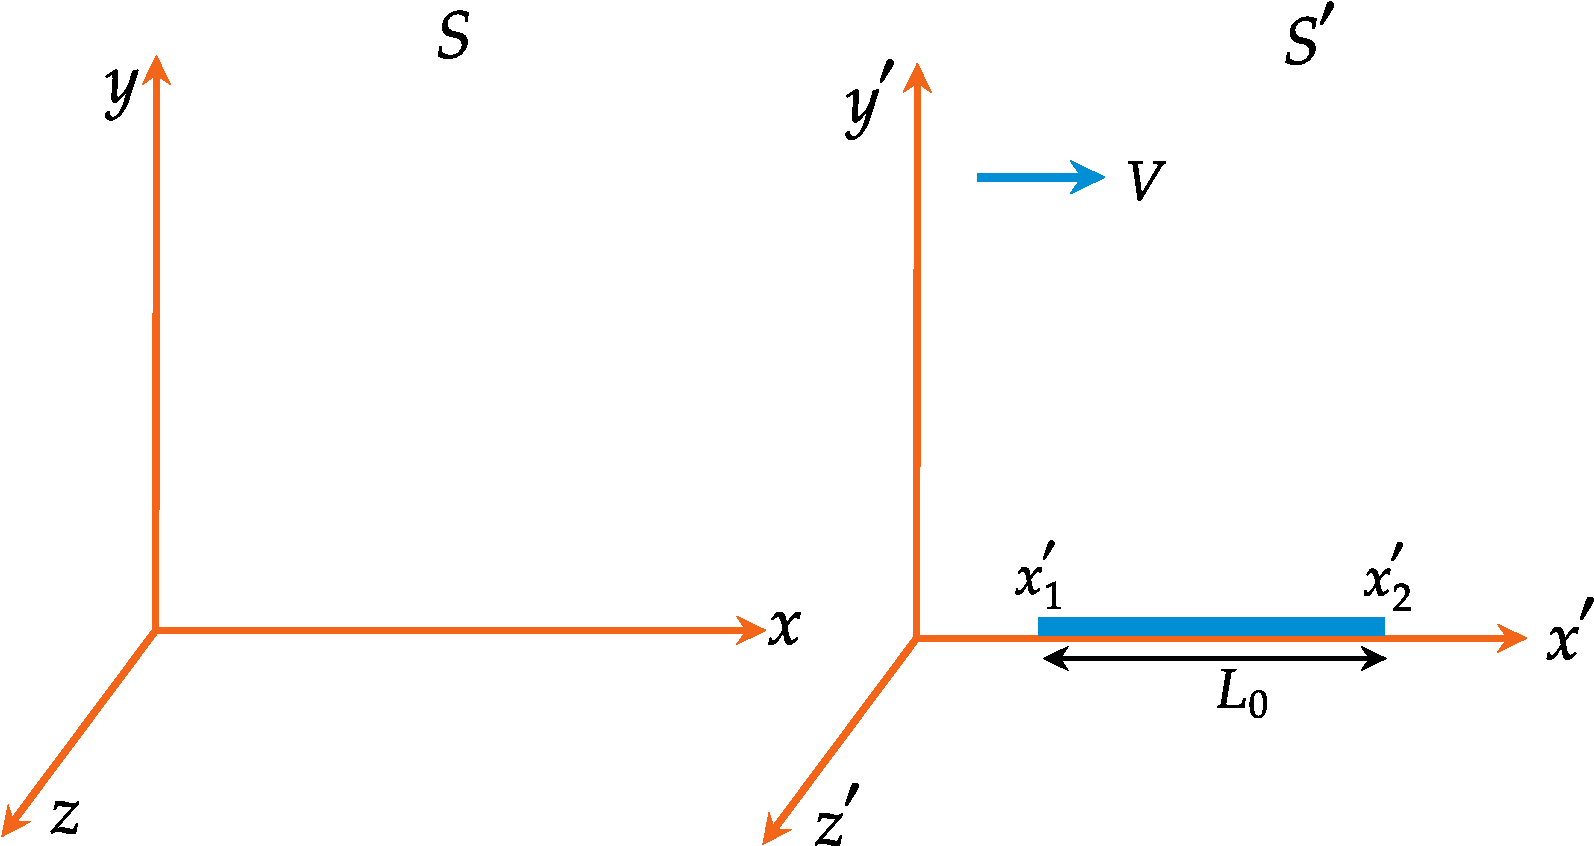
\includegraphics[height=5cm,width=10cm]{length contraction}
	\caption{Length contraction}
	\label{Length contraction}
\end{figure}
If there is a relative motion  between the object and obsever in a system, There will be a discrepancy in measuring it's length .\\
The length $L$ of an object in motion with respect to an observer always appears to the observer to be shorter than it's length $L_{0}$ when it is at rest with respect to the observer. This contraction occurs only in the direction of the relative motion. The length $L_{0}$ of an object in its rest frame is called it's \textbf{proper length}.
\begin{align*}
\intertext { Proper length of rod,} {L}_{0}&=\left({x}_{2}-{x}_{1}\right)\\
\intertext{If $x$ -coordinates of the ends of the rod in reference frame $S^{\prime}$, moving with uniform velocity $v$ with respect to
	frame $\mathrm{S}$ be $\mathrm{x}_{1}^{\prime}$ and $\mathrm{x}_{2}^{\prime}$, as noted simultaneously at same instant $\mathrm{t}^{\prime}$, we have length of rod in moving reference frame $\mathrm{S}^{\prime}$ given by ,}
{L}&=\left({x}_{2}^{\prime}-{x}_{1}^{\prime}\right)
\intertext{According to Lorentz transformation,}
{x}_{1}&=\frac{{{x}_{1}}^{\prime}+{vt}}{\sqrt{1-{v}^{2} / {c}^{2}}} \quad; \quad{x}_{2} =\frac{ {{x}_{2}}^{\prime}+{vt}^{\prime}}{\sqrt{1-{v}^{2} / {c}^{2}}}\\
\text{Then,}\quad L_{0}&=x_{2}-x_{1}\\&=\frac{1}{\sqrt{1-v^{2}  / c^{2}}}\left[x_{2}^{\prime}-x_{1}^{\prime}\right]\\
L_{0}&=\frac{L}{\sqrt{1-v^{2} / c^{2}}}\\
L_{0}&=\gamma L \hspace{2cm} \text{Since,}\ \gamma=\frac{1}{\sqrt{1-v^{2} / c^{2}}}
\end{align*}
\begin{center}
	\framebox{
		\parbox[t][0.8cm]{8cm}{
			
			\addvspace{0.2cm} \centering 
			
			$ L_{0}=\gamma L $ \qquad $\Rightarrow \quad L_{0}=\frac{L}{\sqrt{1-v^{2} / c^{2}}}$} }
\end{center}
\section{Time dilation}
Measurements of time intervals are affected by relative motion between an observer
and what is observed. As a result, a clock that moves with respect to an observer ticks
more slowly than it does without such motion, and all processes  occur more slowly to an observer when they take place in a different inertial frame.\\\\
Let we have two frame of reference, ${S}$ and ${S}^{\prime}$, the former at rest and latter moving with uniform velocity ${v}$, along +ve x-direction.\\
If two events occur at any given point $x$ in frame ${S}^{\prime}$, at time ${t}_{1}^{\prime}$ and $t_{2}^{\prime}$, as noted in the clock carried by it and
at times ${t}_{1}$ and ${t}_{2}$, as noted on the clock carried by frame ${S}$.
\begin{align*}
\intertext{Time interval between two events in frame S,}
\Delta t_{0}&=\left(t_{2}-t_{1}\right)
\intertext{ And we  have time interval between two events, in frame ${S}^{\prime}$}
\Delta t&=\left(t_{2}^{\prime}-t_{1}^{\prime}\right)
\intertext{We have Lorentz transformation equations as, }
t_{1}&=\frac{t_{1}^{\prime}+v_{x}^{\prime} / c^{2}}{\sqrt{1-\frac{v^{2}}{c^{2}}}} \quad ; \quad t_{2}=\frac{t_{2}^{\prime}+v_{x}^{\prime} / t^{2}}{\sqrt{1-v^{2} / c^{2}}}
\intertext{ Then we get the time interval as,}
\Delta t_{0}&=\left(t_{2}-t_{1}\right)\\
&=\frac{t_{2}^{\prime}- t_{1}^{\prime}}{\sqrt{1-v^{2} / c^{2}}}\\&=\frac{\Delta t}{\sqrt{1-v^{2} / c^{2}}}\\
\Delta t_{0}&=\frac{ t_{\text{p}}}{\sqrt{1-v^{2} / c^{2}}}\qquad \Delta t=t_{\text{p}}\\
\Delta t_{0}&=\gamma \ t_{\text{p}}
\end{align*}
Where $t_{\text{p}}$ is the proper time .
\section{Relative velocity}
There is one inertial frame $S, S^{\prime}$ is another inertial frame moving with respect to $S$ in
$x$ -direction and $A$ is another inertial frame which is moving with respect to $S^{\prime}$ with
velocity component $\left(u_{x}^{\prime}, u_{y}^{\prime}, u_{z}^{\prime}\right)$
\begin{align*}
\mathrm{So}, \quad u_{x}^{\prime}&=\frac{d x^{\prime}}{d t^{\prime}} \quad u_{y}^{\prime}=\frac{d y^{\prime}}{d t^{\prime}} \quad u_{z}^{\prime}=\frac{d z^{\prime}}{d t^{\prime}}\\
\intertext{The velocity component of $A$ from $S$ frame is given by,}
u_{x}&=\frac{d x}{d t}, \quad u_{y}=\frac{d y}{d t}, \quad u_{z}=\frac{d z}{d t}
\intertext{ And we  have time interval between two events, in frame ${S}^{\prime}$,}
x&=\gamma\left(x^{\prime}+v t^{\prime}\right), y=y^{\prime}, z=z^{\prime}, t=\gamma\left(t^{\prime}+\frac{v x^{\prime}}{c^{2}}\right)\\\text{Where}\quad \gamma&=\frac{1}{\sqrt{1-\frac{v^{2}}{c^{2}}}}
\intertext { Differentiating both sides, we get ,}
d x&=\gamma\left(d x^{\prime}+v d t^{\prime}\right), \quad d y=d y^{\prime}, \quad d z=d z^{\prime}, \quad d t=\gamma\left(d t^{\prime}+\frac{v d x^{\prime}}{c^{2}}\right)\\
u_{x}&=\frac{d x}{d t}=\gamma\left(\frac{d x^{\prime}+v d t^{\prime}}{d t^{\prime}+\frac{v d x^{\prime}}{c^{2}}}\right)=\frac{\frac{d x^{\prime}}{d t^{\prime}}+v}{1+\frac{v}{c^{2}} \frac{d x^{\prime}}{d t^{\prime}}} \Rightarrow u_{x}=\frac{u_{x}^{\prime}+v}{1+\frac{v}{c^{2}} u_{x}^{\prime}}\\
u_{y}&=\frac{d y}{d t}=\frac{d y^{\prime}}{\gamma\left(d t^{\prime}+\frac{v d x^{\prime}}{c^{2}}\right)}=\frac{\frac{d y^{\prime}}{d t^{\prime}}}{\gamma\left(1+\frac{v}{c^{2}} \frac{d x^{\prime}}{d t^{\prime}}\right)} \quad \Rightarrow u_{y}=\frac{u_{y}^{\prime}}{\gamma\left(1+\frac{v u_{x}^{\prime}}{c^{2}}\right)}\\
u_{z}&=\frac{d z}{d t}=\frac{d z^{\prime}}{\gamma\left(d t^{\prime}+\frac{v d x^{\prime}}{c^{2}}\right)}=\frac{\frac{d z^{\prime}}{d t^{\prime}}}{\gamma\left(1+\frac{v}{c^{2}} \frac{d x^{\prime}}{d t^{\prime}}\right)} \Rightarrow u_{z}=\frac{u_{z}^{\prime}}{\gamma\left(1+\frac{v u_{x}}{c^{2}}\right)}\\
\text { Similarly ,}\quad  u_{x}^{\prime}&=\frac{u_{x}-v}{1-\frac{v u_{x}}{c^{2}}}, \quad u_{y}^{\prime}=\frac{u_{y}}{\gamma\left(1-\frac{v u_{x}}{c^{2}}\right)}, \quad u_{z}^{\prime}=\frac{u_{z}}{\gamma\left(1-\frac{v u_{x}}{c^{2}}\right)}
\end{align*}
\begin{center}
	\framebox{
		\parbox[t][5cm]{4cm}{
			
			\addvspace{0.2cm} \centering 
		\begin{align*}
		u_{x}&=\frac{u_{x}^{\prime}+v}{1+\frac{v}{c^{2}} u_{x}^{\prime}}\\
		u_{y}&=\frac{u_{y}^{\prime}}{\gamma\left(1+\frac{v u_{x}^{\prime}}{c^{2}}\right)}\\
		u_{z}&=\frac{u_{z}^{\prime}}{\gamma\left(1+\frac{v u_{x}}{c^{2}}\right)}
		\end{align*}
			} }
\end{center}
\section{Relativistic mass}
The mass of a body moving at the speed v relative to an observer is larger than its mass when at rest relative to the observer by the factor, $\frac{1}{\sqrt{1-\frac{v^{2}}{c^{2}}}}$
\begin{align*}
\text { Thus } \quad m&=\frac{m_{0}}{\sqrt{1-\frac{v^{2}}{c^{2}}}}
\intertext{Where $m_{0}$ is rest mass of body and $\mathrm{m}$ is observed mass.}
\end{align*}
\subsection{Relativistic momentum}
$$
p=m v=\frac{m_{0} v}{\sqrt{1-\frac{v^{2}}{c^{2}}}}
$$
\subsection{Relativistic energy}
Einstein suggested if m is relativistic mass of body then relativistic energy E is given
by,
$$
E=m c^{2} \quad \text { and } \quad E=\frac{m_{0} c^{2}}{\sqrt{1-\frac{v^{2}}{c^{2}}}}
$$

		

\newpage
\begin{abox}
	Practise Set-3
\end{abox}
\begin{enumerate}[ label=\color{ocre}\textbf{\arabic*.}]

	\item Suppose you are driving your car on a business trip and are traveling at $30 \mathrm{~m} / \mathrm{s}$. Your boss, who is waiting at your destination, expects the trip to take $5.0 \mathrm{~h}$. When you arrive late, your excuse is that your car clock registered the passage of $5.0 $ \ but that you were driving fast and so your clock ran more slowly than your boss's clock. If your car clock actually did indicate a $5.0-\mathrm{h}$ trip, how much time passed on your boss's clock, which was at rest on the Earth?
	\begin{answer}
		\begin{align*}
		\text{	Here, }\quad \gamma&=\frac{1}{\sqrt{1-v^{2} / c^{2}}}=\frac{1}{\sqrt{1-\frac{\left(3 \times 10\  \text{m}/\text{s}^{2}\right)}{\left(3 \times 10^{8} \mathrm{~m} / \mathrm{s}^2\right)}}}\\&=\frac{1}{\sqrt{1-10^{-14}}}
		\intertext{Perform binomial expansion, we get}
		\gamma&=\left(1-10^{-14}\right)^{-1 / 2} \approx 1+\frac{1}{2}\left(10^{-14}\right)=1+\frac{1}{2}\left(10\times 10^{-15}\right) \\&=1+5 \times 10^{-15}
		\intertext{In daily life, $\gamma$ is not much different from $1$.}
		\Delta t&=\gamma \Delta t_{p}\\&=\left(1+5 \times 10^{-15}\right)(5.0 \text{h})=5.0 \text{h}+2.5 \times 10^{-14} \text{h}\\&=5\text{h}+0.09 \mathrm{ns}
		\intertext{Your boss's clock would be only $0.09 \mathrm{~ns}$ ahead of your car clock. }
		\end{align*}
	\end{answer}
	
	\item Imagine a motorcycle moving with a speed $0.80 \mathrm{c}$ past a stationary observer. If the rider tosses a ball in the forward direction with a speed of $0.70 \mathrm{c}$ relative to himself, what is the speed of the ball relativeto the stationary observer?
	\begin{answer}
		\begin{align*}
		\intertext{	The speed of the motorcycle relative to the stationary observer is,} v&=0.8 \mathrm{c}\intertext{The speed of the ball in the frame of reference of the motorcyclist is,}  u_{x}^{\prime}&=0.7 \mathrm{c} . \intertext{Therefore, the speed,$\mathrm{u}_{x}$ of the ball relative to the stationary observer is,}
		u_{x}&=\frac{u_{x}^{\prime}+v}{1+\frac{u_{x}^{\prime} v}{c^{2}}}\\&=\frac{0.70 c+0.80 c}{1+\frac{(0.70  c)(0.80 c)}{c^{2}}}\\&=0.96 c
		\end{align*}
	\end{answer}
	\item An electron, which has a mass of $9.11 \times 10^{31} \mathrm{~kg}$, moves with a speed of $0.750 \mathrm{c}$. Find its relativistic momentum.
	\begin{answer}
		\begin{align*}
		p&=\frac{m_{e} v}{\sqrt{1-\frac{v^{2}}{c^{2}}}}\\
		&=\frac{\left(9.11 \times 10^{-31} \mathrm{~kg}\right)\left(0.750 \times 3.00 \times 10^{8} \mathrm{~m} / \mathrm{s}\right)}{\sqrt{1-\frac{(0\cdot750c)^{2}}{c^{2}}}}\\&=3.10 \times10^{-22} kg\ m/s
		\end{align*}
	\end{answer}
	\item An electron in a television picture tube typically moves with a speed $u=0.25 c$.  Find its total energy and kinetic energy in electron volts.
	\begin{answer}
		\begin{align*}
		\intertext{	Rest energy of electron is $0.511 \mathrm{MeV}$}
		E&=\frac{m_{e} c^{2}}{\sqrt{1-\frac{u^{2}}{c^{2}}}}\\&=\frac{0.511 \mathrm{MeV}}{\sqrt{1-\frac{(0.250 c)^{2}}{c^{2}}}}\\
		&=0.528 \mathrm{MeV}
		\intertext{This is $3 \%$ greater than the rest energy.}
		\intertext{We obtain the kinetic energy by subtracting the rest energy from the total energy:}
		K&=E-m_{e} c^{2}\\&=0.528 \mathrm{MeV}-0.511 \mathrm{MeV}\\&=0.017 \mathrm{MeV}
		\end{align*}
	\end{answer}
	\item (a) Find the rest energy of a proton in electron volts.
	\\(b) If the total energy of a proton is three times its rest energy, with what speed is the proton moving?
	\\(c) Determine the kinetic energy of the proton in electron volts.

	\begin{answer}
		\begin{align*}
		\text{(a)}\quad E_{R}&=m_{p} c^{2}\\&=\left(1.67 \times 10^{-27} \mathrm{~kg}\right)\left(3.00 \times 10^{8} \mathrm{~m} / \mathrm{s}\right)^{2}\\
		&=\left(1.50 \times 10^{-10} J\right)\left(1.00 \mathrm{eV} / 1.60 \times 10^{-19} J\right)\\&=938 \mathrm{MeV}\\\\
		\text{(b)}\quad E&=3 m_{p} c^{2}=\frac{m_{p} c^{2}}{\sqrt{1-\frac{u^{2}}{c^{2}}}} \quad \\3&=\frac{1}{\sqrt{1-\frac{u^{2}}{c^{2}}}}\\
		\text{Solving }&\text{for $'u'$ gives}\\
		1-\frac{u^{2}}{c^{2}}&=\frac{1}{9} \quad \\ \frac{u^{2}}{c^{2}}&=\frac{8}{9}  \\ u&=\frac{\sqrt{3}}{8} c\\&=2.83 \times 10^{8} \mathrm{~m} / \mathrm{s}\\\\
		\text{(c)}\quad K&=E-m_{p} c^{2}\\&=3 m_{p} c^{2}-m_{p} c^{2}=2 m_{p} c^{2}\\
		\text{Because,}\ m_{p} c^{2}&=938 \mathrm{MeV},\\ K&=1.880 \mathrm{MeV}
		\end{align*}
	\end{answer}
	\item A rigid bar of length $1.5 \mathrm{~m}$ is at rest relative to frame $S^{\prime}$. If it makes an angle $\alpha^{\prime}=45^{\circ}$ with $x^{\prime}-$ axis, find the length of the bar and its orientation relative to frame $S$, when $v=0.95 c ?$
	\begin{answer}
		\begin{align*}
		\intertext{Resolving the length of the bar into components parallel to $x^{\prime}$ and $y^{\prime}$ axes, the corresponding length in $S^{\prime}$ are:}
		L_{x}^{\prime}&=L^{\prime} \cos \alpha^{\prime}=1.5 \times 1 / \sqrt{2}=1.06m;\\L_{y}^{\prime}&=L^{\prime}\sin \alpha^\prime-1.5\times1/\sqrt{2}=1.06m
		\intertext{The vertical components would show no contraction, when viewed from $S$ Horizontal component, being parallel to $v$, would}
		\therefore \quad L_{y}&=L_{y}^{\prime}=1.06 m\\
		L_{x}&=L_{x}^{\prime} \sqrt{1-v^{2} / c^{2}}=1.06 \sqrt{1-0.95^{2}}-0.331 m
		\intertext{Therefore, length of the relative $S$ is:}
		L_{1}&=\sqrt{L_{x}^{2}+L_{y}^{2}}=\sqrt{(1.06)+(0.331)}=1.11 \mathrm{~m}\\
		\intertext{	Orientation of the bar relative to $S$ is}
		\tan \alpha&=\frac{L_{y}}{L_{x}}=\frac{1.06}{0.331}=3.20 \quad \\\therefore \alpha&=72^{\circ} 40^{\prime}
		\end{align*}
	\end{answer}
	\item An experimental intends to study a beam of $\pi$ -mesôns of velocity $0.9 c$. How far can he place his apparatus from the target where $\pi$ -measons are produced and still expect to get-sufficient number of $\pi$ -mesons.
	\begin{answer}
		\begin{align*}
		\intertext{ With relativistic time dilation,}
		\Delta t&=\Delta t^{\prime} / \sqrt{1-0.9^{2}}=2.3 \Delta t^{\prime}
		\intertext{Since $\Delta t^{\prime}$ is the time-interval measured by an observer moving with $\pi$ -mesons, it is the real life-time, so that}
		\intertext{$\Delta t^{\prime}=2 \times 10^{-8} s .$ So, in the lab-frame, the mean life is}
		\Delta t&=2.3 \times \Delta t^{\prime}=2.3 \times 2 \times 10^{-8} s\\&=4.6 \times 10^{-8} s
		\intertext{Therefore, average distance travelled by $\pi$ -mesons }&=v . \Delta t=0.9 \times 3 \times 10^{8} \times 4.6 \times 10^{-8} \\\mathrm{~m}&=12.42 \mathrm{~m}
		\end{align*}
	\end{answer}
	\item The half-life of a particular particle as measured in the lab is $4.0 \times 10^{-8} s$ whęn its speed is $0.80 \mathrm{c}$ and $3 \times 10^{-8} s$ when its speed is $0.60 \mathrm{c}$. Find its actual life time.
	\begin{answer}
		\begin{align*}
		\intertext{Due to time-dilation, the half-life of a moving particle appears lengthened. Let $\Delta t_{0}$ be the actual half-life, i.e.,in the frame of reference of the particle, and $\Delta t$ that measured by a stationary observer.}
		\therefore \quad \Delta t&=\Delta t_{0} / \sqrt{1-v^{2} / c^{2}}\\
		\intertext{Therefore, by the problem}
		4.0 \times 10^{-8}&=\frac{\Delta t}{\sqrt{1-0.8^{2}}} ; 3.0 \times 10^{-8}=\frac{\Delta t_{0}}{\sqrt{1-0.6^{2}}}
		\intertext{Either relation gives, $\Delta t_{0}=2.4 \times 10^{-8} s$, the actual life-time.}
		\end{align*}
	\end{answer}
	\item What will be the period of the 'seconds' pendulum measured by an observer moving with a speed of $0.8 \mathrm{c}$ ?
	\begin{answer}
		\begin{align*}
		\intertext{If $T_{0}(=2 s)$ be the period of a seconds pendulum asmeasured by an observer at rest, the same would be, say To the moving observer}
		\intertext{Therefore, from the time-dilation relation,}
		T&=\frac{T_{0}}{\sqrt{1-v^{2} / c^{2}}}=\frac{2}{\sqrt{1-0.8^{2}}}=3.33 s
		\end{align*}
	\end{answer}
	\item The average life-time of neutron is $5$min. It disintegrates spontaneously in to an electron,a proton and a neutrino. Ifthe distance of the sun from the earth is $11 \times 10^{10} m_{i}$ find the average minimum velocity with which a neutron must leave the sun so.as to reach the earth before breaking up.
	\begin{answer}
		\begin{align*}
		\intertext{Let $v$ be the required velocity of the neutron. The time $t_{1}$ for neutron to reach the earth from the sun before decay is}
		t_{1}&=\frac{11 \times 10^{10} m}{v}\\
		\intertext{If $t_{0}$ be the life-time of neutron at rest, then the average life-time $t$ of the 'moving' neutro, as measured by an observer on earth, is}
		t&=\frac{t_{0}}{\sqrt{1-v^{2} / c^{2}}}=\frac{15 \times 60 s}{\sqrt{1-v^{2} / c^{2}}}
		\intertext{Plainly, this $t$ and previous $t_{1}$ must be equal,}
		\therefore \quad \frac{11 \times 10^{10}}{v}&=\frac{15 \times 60}{\sqrt{1-v^{2} /\left(3 \times 10^{8}\right)^{2}}}
		\intertext{Simplifying, we obtain,}
		v&=1.132 \times 10^{8} \mathrm{~ms}^{-1}
		\end{align*}
	\end{answer}
	\item A rocket is travelling towards the moon with a velocity $0.6 \mathrm{c}$. When half-way to the moon, it fires a message rocket back towards the earth with a velocity $0.8 \mathrm{c}$ relative to the primary rocket. What a velocity of the message rocket as seen by a terrestrial observer? Neglect the recoil.
	\begin{answer}
		\begin{align*}
		\intertext{The velocity of the message rocket relative to a terrestrial observer is, by velocity addition theorem,}
		v&=\frac{(0.6-0.8) c}{1-0.8 \times 0.6}=\frac{-0.2 c}{1-0.48}\\
		&=-\frac{0.2 c}{0.52}\\&=-0.385 c
		\intertext{The negative sign indicates that the rocket is moving towards the earth.}
		\end{align*}
	\end{answer}

\item How many years does it take for an atomic clock (with a precision of one part over $10^{15}$ ), which is placed at rest on Earth, to lose one second with respect to an identical clock placed on the Sun? (Hint: apply Lorentz transformations as if both reference frames were inertial, with a relative velocity $v \simeq 310^{4} \mathrm{~m} / \mathrm{s} \simeq 10^{-4} \mathrm{c}$ ).
\begin{answer}
	\begin{align*}
	\text{Setting,}\ \Delta t&=1s\\ \text{We have,}\ T&=\frac{\Delta t}{\left(1-\sqrt{1-v^{2} / c^{2}}\right)} \\& \simeq 2 \Delta t \frac{c^{2}}{v^{2}}\\& \simeq 6.34 \text{years.}
	\end{align*}
\end{answer}
\end{enumerate}



